\chapter{Literature Review}
\label{chap3}

\section{Related Problems}
The unshredding problem can be viewed as a special case of the general jigsaw reconstruction problem. Automatically solving jigsaws has been an active area of research since the 60s \cite{P21} and as such there is a wealth of information published on this topic. However the majority of early methods focus entirely on the shape information of the pieces (eg: \cite{P21,P22}) and are therefore not applicable to our problem. More recently there have been several attempts that also utilise the visual information of the pieces (eg: \cite{P23,P24}), however these methods mostly focus on the distribution of colours on the images and thus are not easily applicable to our black and white domain. Additionally, the solutions proposed are generally restricted to very small problem instances (usually less than 50 pieces), which is too small a number for our purposes. One promising method is presented in \cite{P25}. Here the authors reconstruct the jigsaw while looking only at image features, and also manage to solve instances with as many as 320 pieces. The features used in their comparison function are viable candidates for shred comparison or clustering.

Another related problem is the reconstruction of full-colour shredded documents. As opposed to the jigsaw puzzle formulation, this problem has no edge shape information to use. However, the availability of full-colour means that the amount of information available on a shred is much higher than in the case of binary data (i.e. black and white pixels). A thorough review of this problem is presented in \cite{P26}. Here, Skeoch analyses several types of distance functions that look at how similar two pixels are and uses these to design some simple yet effective shred comparison functions. However, the author notes that these methods don't work very well on black and white documents. Additionally, the analysis is restricted to the strip-cut variant.

Yet another related problem, is the reconstruction of hand-torn documents. In this problem, edge shape becomes once more a big factor, especially since hand-torn documents tend to contain much fewer shreds than mechanically torn ones. Most approaches (eg: \cite{P18,P27,P31}) focus on curve matching methods and are therefore not applicable to us. Additionally, since the search space is smaller, such approaches are generally quite computationally expensive (\cite{P18}, for instance, was only tested on up to 15 shreds). One interesting method in this area was presented by De Smet in \cite{P30}. Here, he proposes a search algorithm that takes advantage of the way humans tend to stack hand-torn shreds and which successfully manages to speed up the search process. A method more applicable to our problem is analysed in \cite{P32}, where the authors look at the effectiveness of different features when used to cluster the shreds based on similarity.

A final related problem is the \emph{semi-automatic} reconstruction of shredded documents. Some of the most successful reconstruction methods developed so far, including those that won the DARPA Shredder Challenge \cite{P33,P34} fall under this category and incorporate human input into the evaluation loop. Using even a small amount of human expertise can vastly reduce the difficulty of the problem, because humans can catch errors early, before these have a chance to propagate. One example of such a system is shown in Figure \ref{fig:deshredder}

\begin{figure}[h]
    \centering
    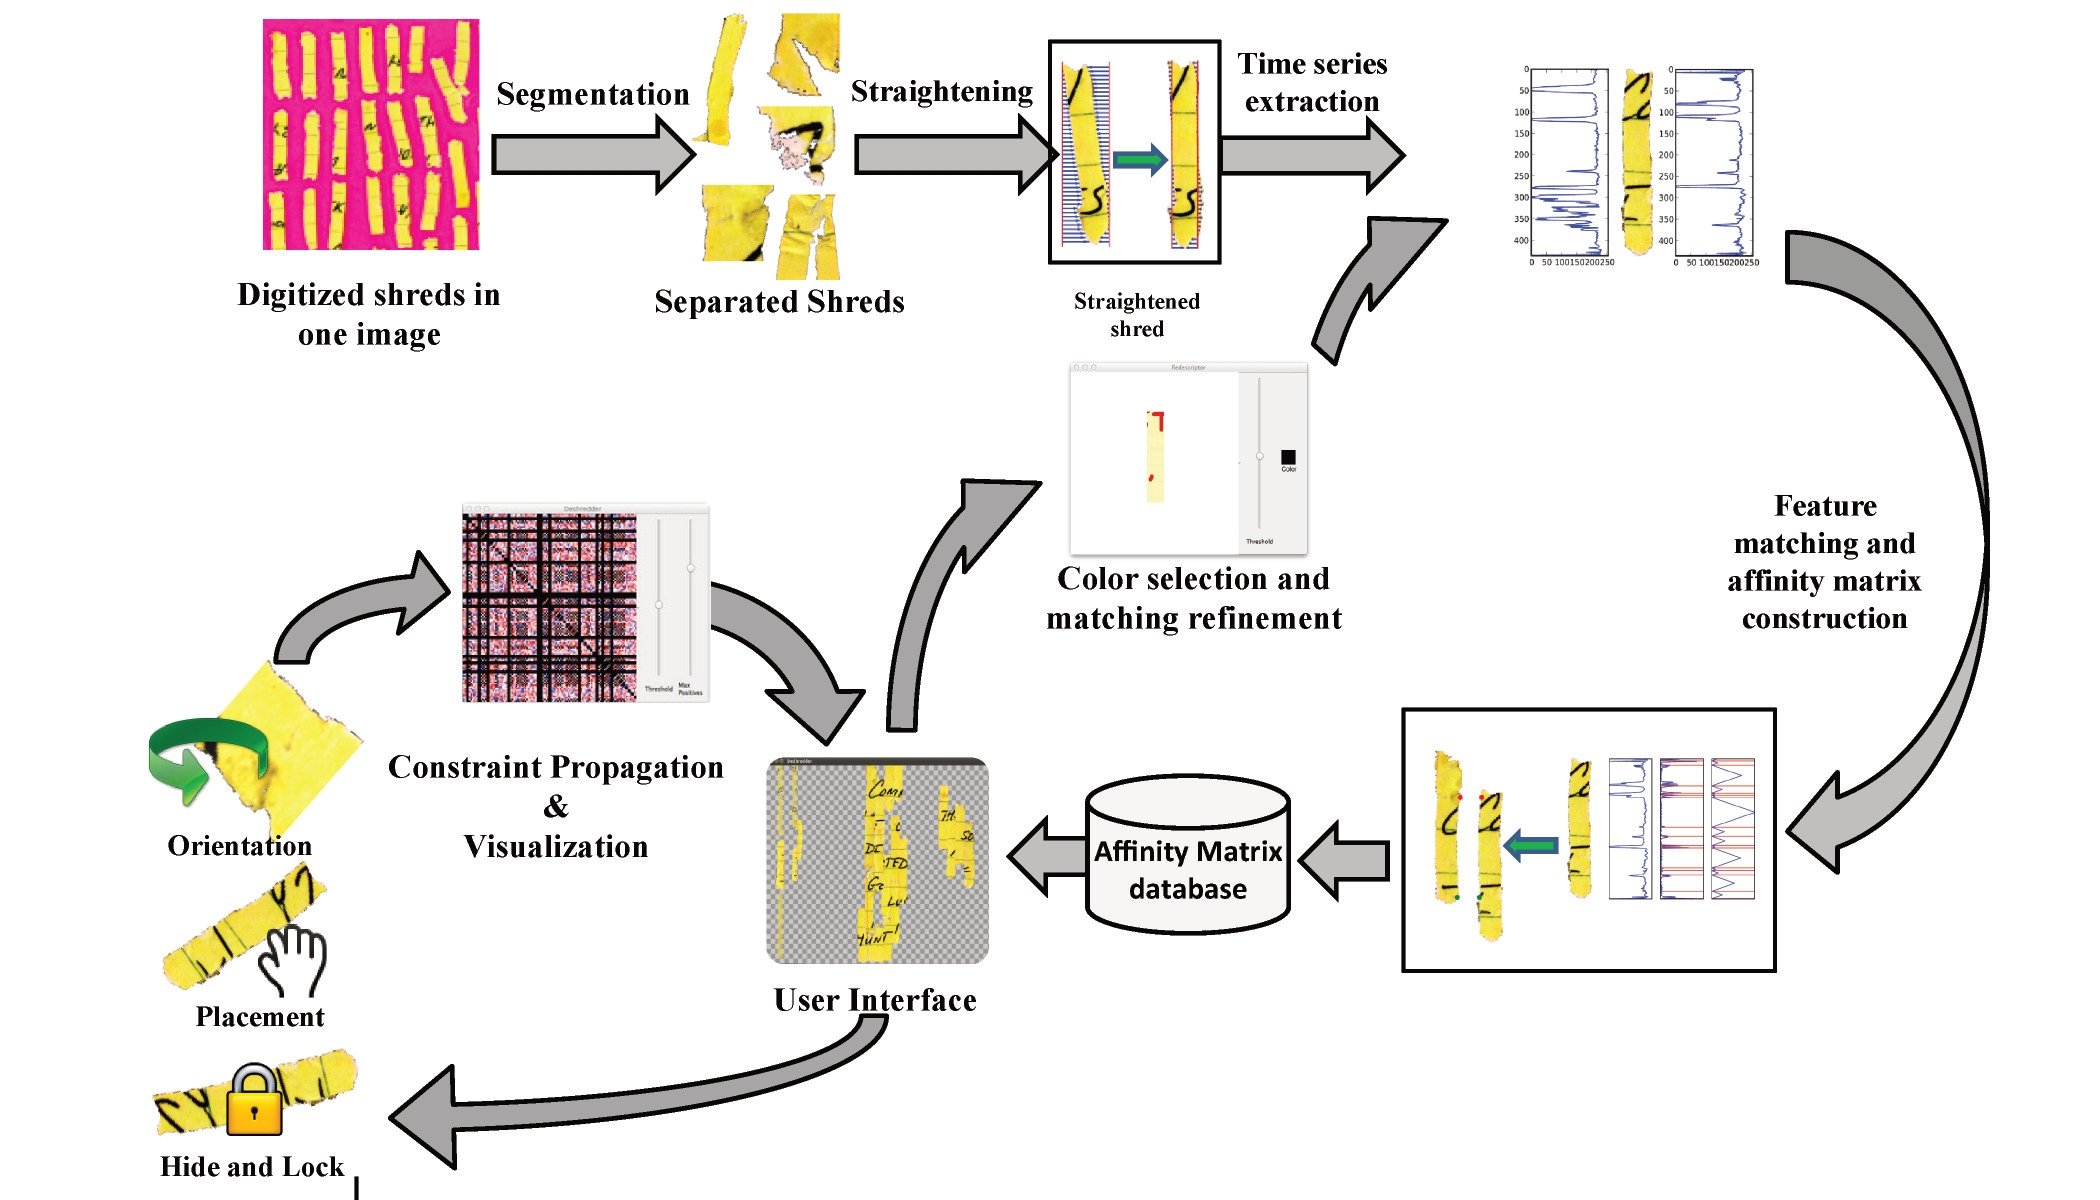
\includegraphics[width=\textwidth]{deshredder.jpg}
    \caption{The pipeline of the Deshredder algorithm and user interface. Figure taken from \cite{P34}.}
    \label{fig:deshredder}
\end{figure}

A particularly interesting semi-automatic approach was developed in \cite{P35}, where the authors show a shred to the user and then allow him to draw what a portion of the neighbouring shred might look like. The user is then shown shreds which match his drawing, at which point he can either select a correct match from the proposed edges or decide change his drawing.

\clearpage

\section{Edge comparison functions}
Most previously published approaches have used a \emph{cost} function to compare edge matches. A cost function means that a lower cost represents a better match and, in particular, a cost of $0$ shows a perfect match and a cost of $\infty$ shows an impossible one. 

Relatively little progress has been made in developing the cost function. Most papers (eg: \cite{P1,P5,P6,P7,P20,P36}) settle on a simple ``Gaussian cost" formulation which does a weighted difference of each pair of adjacent pixels on either side of the proposed join and increases the cost of the join if the pixels are too dissimilar. The logic here is that neighbouring shreds are more likely to have matching pixels on their edges. In order to mitigate the effect of noise, a ``Gaussian" comparison is done by looking at a small neighbourhood of pixels rather than doing a single pixel to pixel comparison (see Figure \ref{fig:gausIdea}).

\begin{figure}[h]
    \centering
    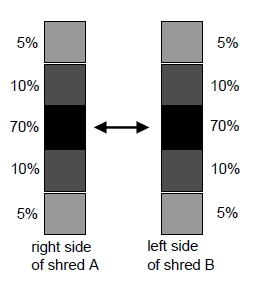
\includegraphics[width=0.5\textwidth]{gausIdea}
    \caption{Cost function calculating the weighted sum of the difference between two opposing pixels and their respective opposing neighbours. Figure taken from \cite{P20}}
    \label{fig:gausIdea}
\end{figure}

In order to formally define this function, we first must get a term for the weighted sum of the $y$th pixel on shred A being matched to the corresponding $y$th pixel on shred B. We call this function $e'_h(A,B,y)$ and define it as: 
\begin{equation*}
\begin{split}
e'_h(A,B,y) = &  |0.7(v_r(A,y) - v_l(B,y)) + \\ 
              &  0.1(v_r(A,y+1) - v_l(B,y+1)) + \\
              &  0.1(v_r(A,y-1) - v_l(B,y-1)) + \\
              &  0.05(v_r(A,y+2) - v_l(B,y+2)) + \\
              &  0.05(v_r(A,y-2) - v_l(B,y-2))|
\end{split}
\end{equation*}
where $v_r(A,y)$ returns the $y$th pixel on the right edge of shred $A$ and $v_l(A,y)$ returns the $y$th pixel on the left edge of shred $A$.

Once we have this weighted sum, we can pass it through a threshold $\tau$ in order to obtain the pixel cost: 
\[ e_h(A,B,y) = \left\{
	\begin{array}{ll}
		1 \mbox{ if } e'_h(A,B,y) \geq \tau \\
		0 \mbox{ otherwise }
	\end{array}
\right. \]

And finally, the edge cost is simply the sum of all pixel costs:
\[c_r(A,B) = \sum_{y \in \mbox{\small Edge Pixels}} e_h(A,B,y) \]

One problem with the above formulation is that matching a completely white edge to another completely white edge will give a perfect cost of 0. Therefore whenever such a white-on-white match is available it will be taken, which can result in undesirable behaviour (see Figure \ref{fig:white}).

\begin{figure}[h]
    \centering
    
\includegraphics[width=\textwidth]{white}
    \caption{{\bf Left:} the correct match. {\bf Right:} white-on-white match which would get a perfect cost under the Gaussian cost function and be incorrectly preferred}
    \label{fig:white}
\end{figure}

A refinement to the cost function that solves the white-on-white problem is proposed in \cite{P2}. Here, the authors base the cost only on how well the black pixels match (i.e they disregard matching white pixels from their cost computation). This paper also introduces a heuristic that penalises edges that have too few black pixels on them. These improvements result in the best cost function published so far and therefore the main benchmark against which we will compare our method. 

The authors of \cite{P8} present another proof-of-concept cost function improvement. They use computer vision techniques to identify individual characters that were split between different shreds and try to match them together. The authors learn the correct character shapes from the shreds themselves, therefore the method can be applied on any character set. The paper has promising preliminary results but doesn't provide comparisons with other cost functions, so aspects such as robustness to noise remain unclear.

\clearpage
\section{Search functions}
\label{chap2Search}
Significant effort has been made towards finding a good search function and several different approaches have been explored.  In \cite{P1}, the authors show that the search problem is NP hard by reducing it to a Travelling Salesman Problem. The authors then solve this Travelling Salesman Problem by using the Chained Lin-Kernighan heuristic \cite{P37}.  In \cite{P6} an exact solution is attempted via Integer Linear Programming. Due to the large search space, this paper only looks at the strip-cut variant. The method presented here yields very good results but is intractable for any number of strips above 150. This suggests that any attempts to use Integer Linear Programming for the cross-cut variant would likely be futile. 

Several attempts at using top-down local improvement have also been made. These methods first obtain a seed solution using a heuristic function and then attempt to improve upon this solution via local search methods. In \cite{P5} the authors apply the Variable Neighbourhood Search meta-heuristic \cite{P38}, which contains two parts, a local search function called variable neighbourhood descent and a perturbation function which aims to help the local search escape local optima. The variable neighbourhood descent searches neighbourhoods of increasing size for a solution that is better than the current one. Here neighbourhoods are obtained by either swapping single pieces, or shifting groups of pieces around. The perturbation function simply adds some randomness in the form of occasionally switching the solution to a neighbour even if the neighbour's score is worse than our current score. In the same paper, the authors also define an Ant Colony Optimization solution \cite{P39}. This Ant Colony Optimization formulation proved to be overall better than the Variable Neighbourhood Search heuristic, but at the cost of a longer runtime. These results are improved upon in \cite{P7}, where the authors use the same Variable Neighbourhood Search formulation, but embed it into a genetic algorithm. The method defines several mutation and recombination operators which are applied to an initial population of solutions generated by some simple heuristics. Between every step of the genetic algorithm, the solution pool is improved by running the Variable Neighbourhood Search algorithm.

As mentioned above, \cite{P5,P7} both rely on heuristic search methods to provide them with initial seed solutions. One of these methods is the Row Building Heuristic (RBH). RBH tries to take advantage of the fact that shreds with a completely white edge probably belong on the margin of the document. RBH therefore randomly selects a shred with a white left edge as its starting shred. It then adds the best match, as defined by the cost function, to the right of this starting edge. The greedy process is repeated, thus increasing the length of the current row, until we append a piece which has a white right edge, at which point the algorithm simply restarts and attempts to build the next row. 

The second heuristic worth mentioning is the Prim Based Heuristic, which is analogous to the Prim minimum spanning tree algorithm \cite{P40}. This works by picking a random shred as a starting point and then expanding it by adding a shred to one of the four possible neighbouring positions. The process is repeated, always greedily adding the best edge to one of the neighbours of our current solution (see Figure \ref{fig:prim}). 
\begin{figure}[H]
        \centering
        \begin{subfigure}[b]{0.45\textwidth}
                \centering
                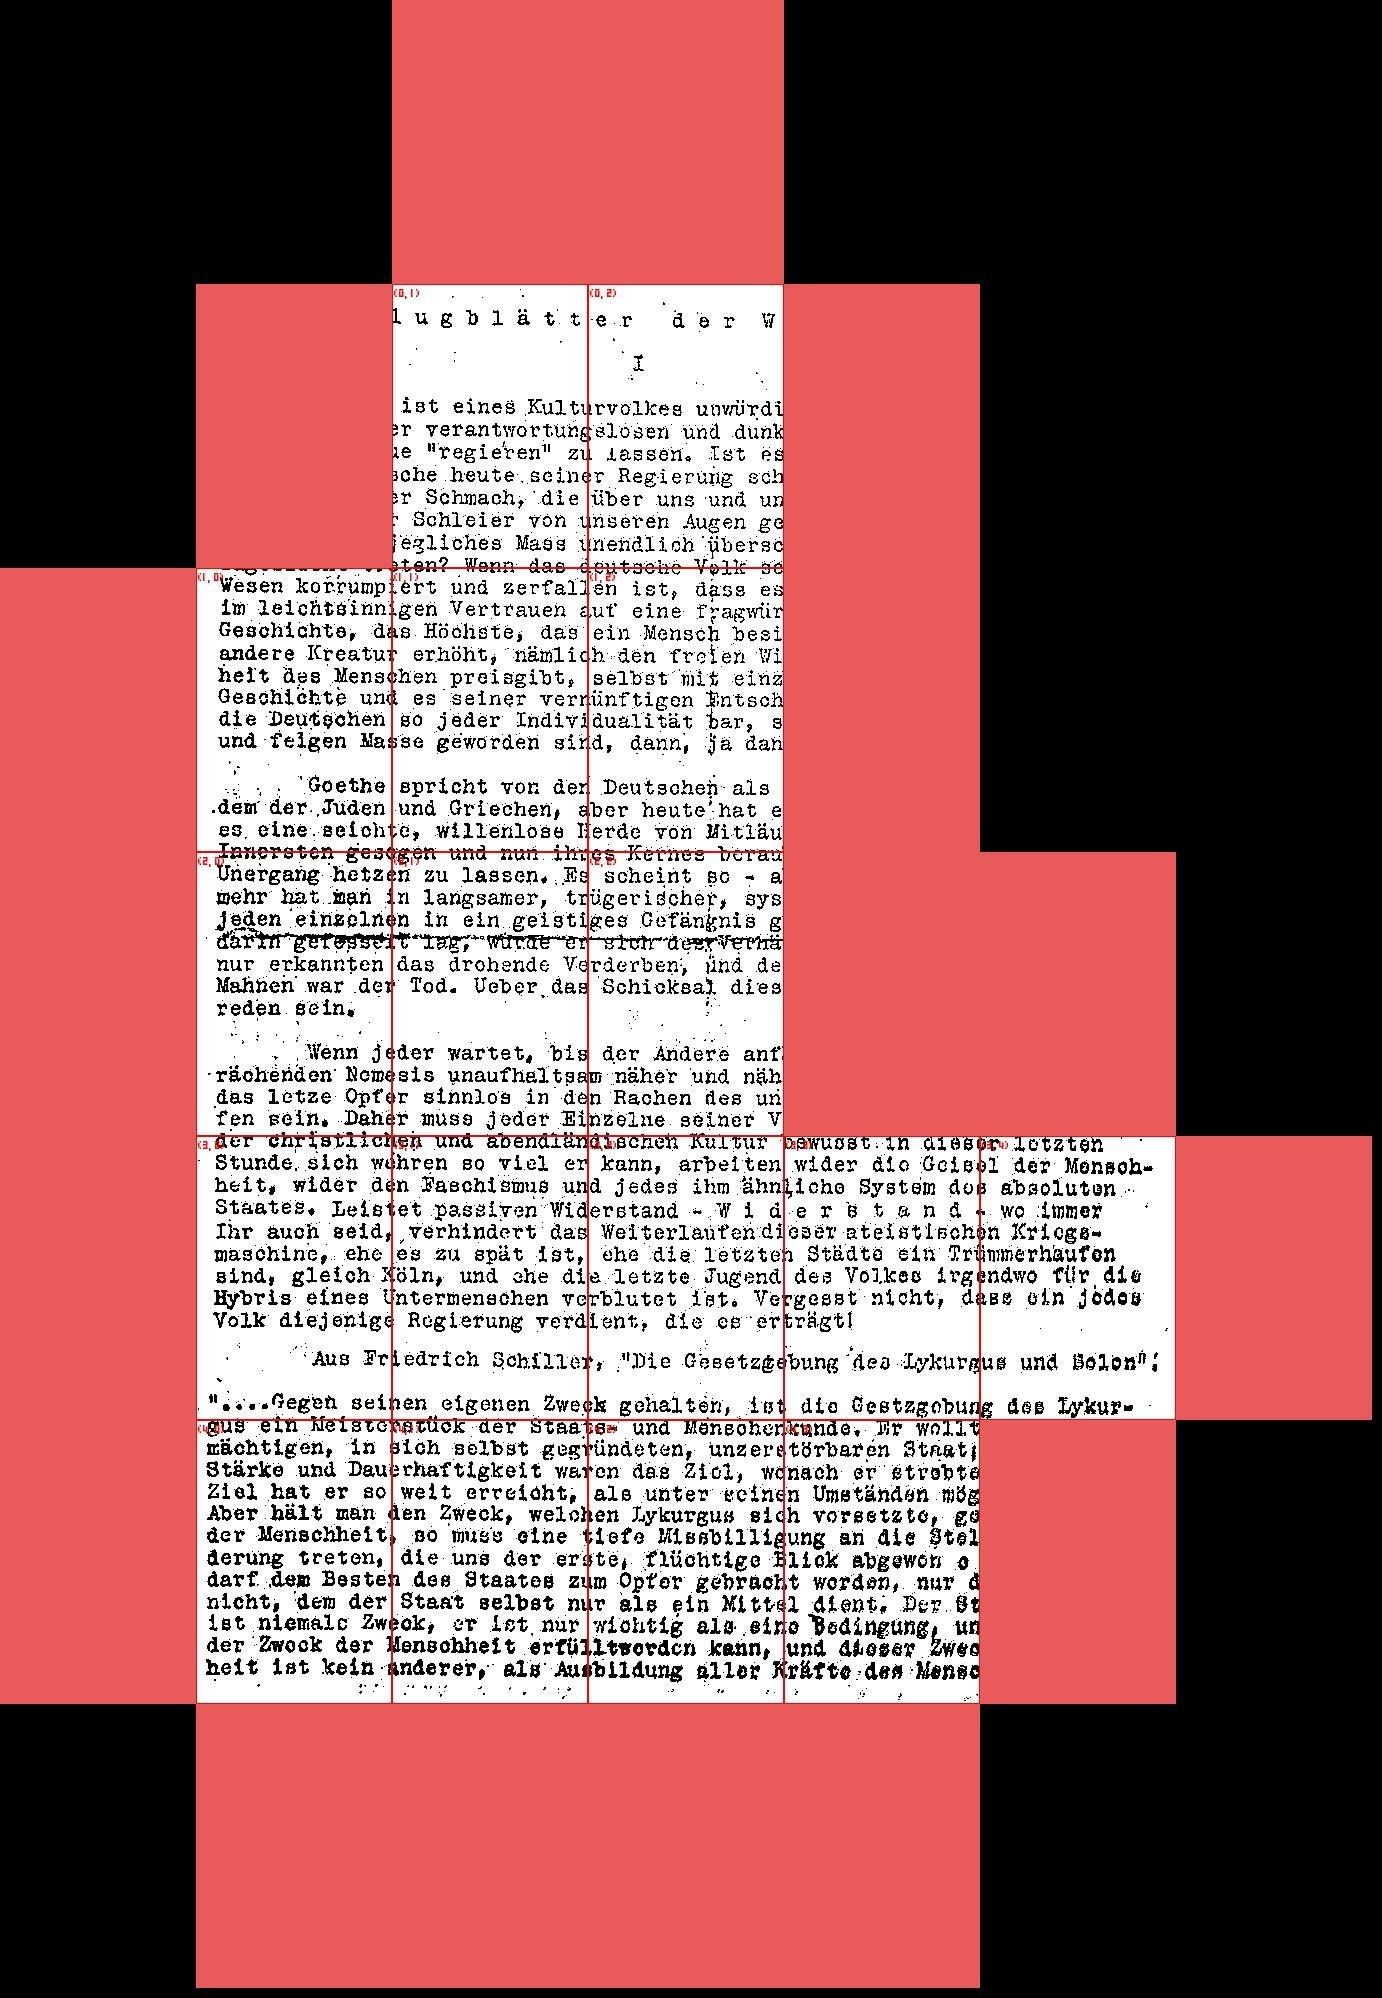
\includegraphics[width=\textwidth]{prim1}
                \vspace{0.3em}
        \end{subfigure}
        ~ 
        \begin{subfigure}[b]{0.45\textwidth}
                \centering
                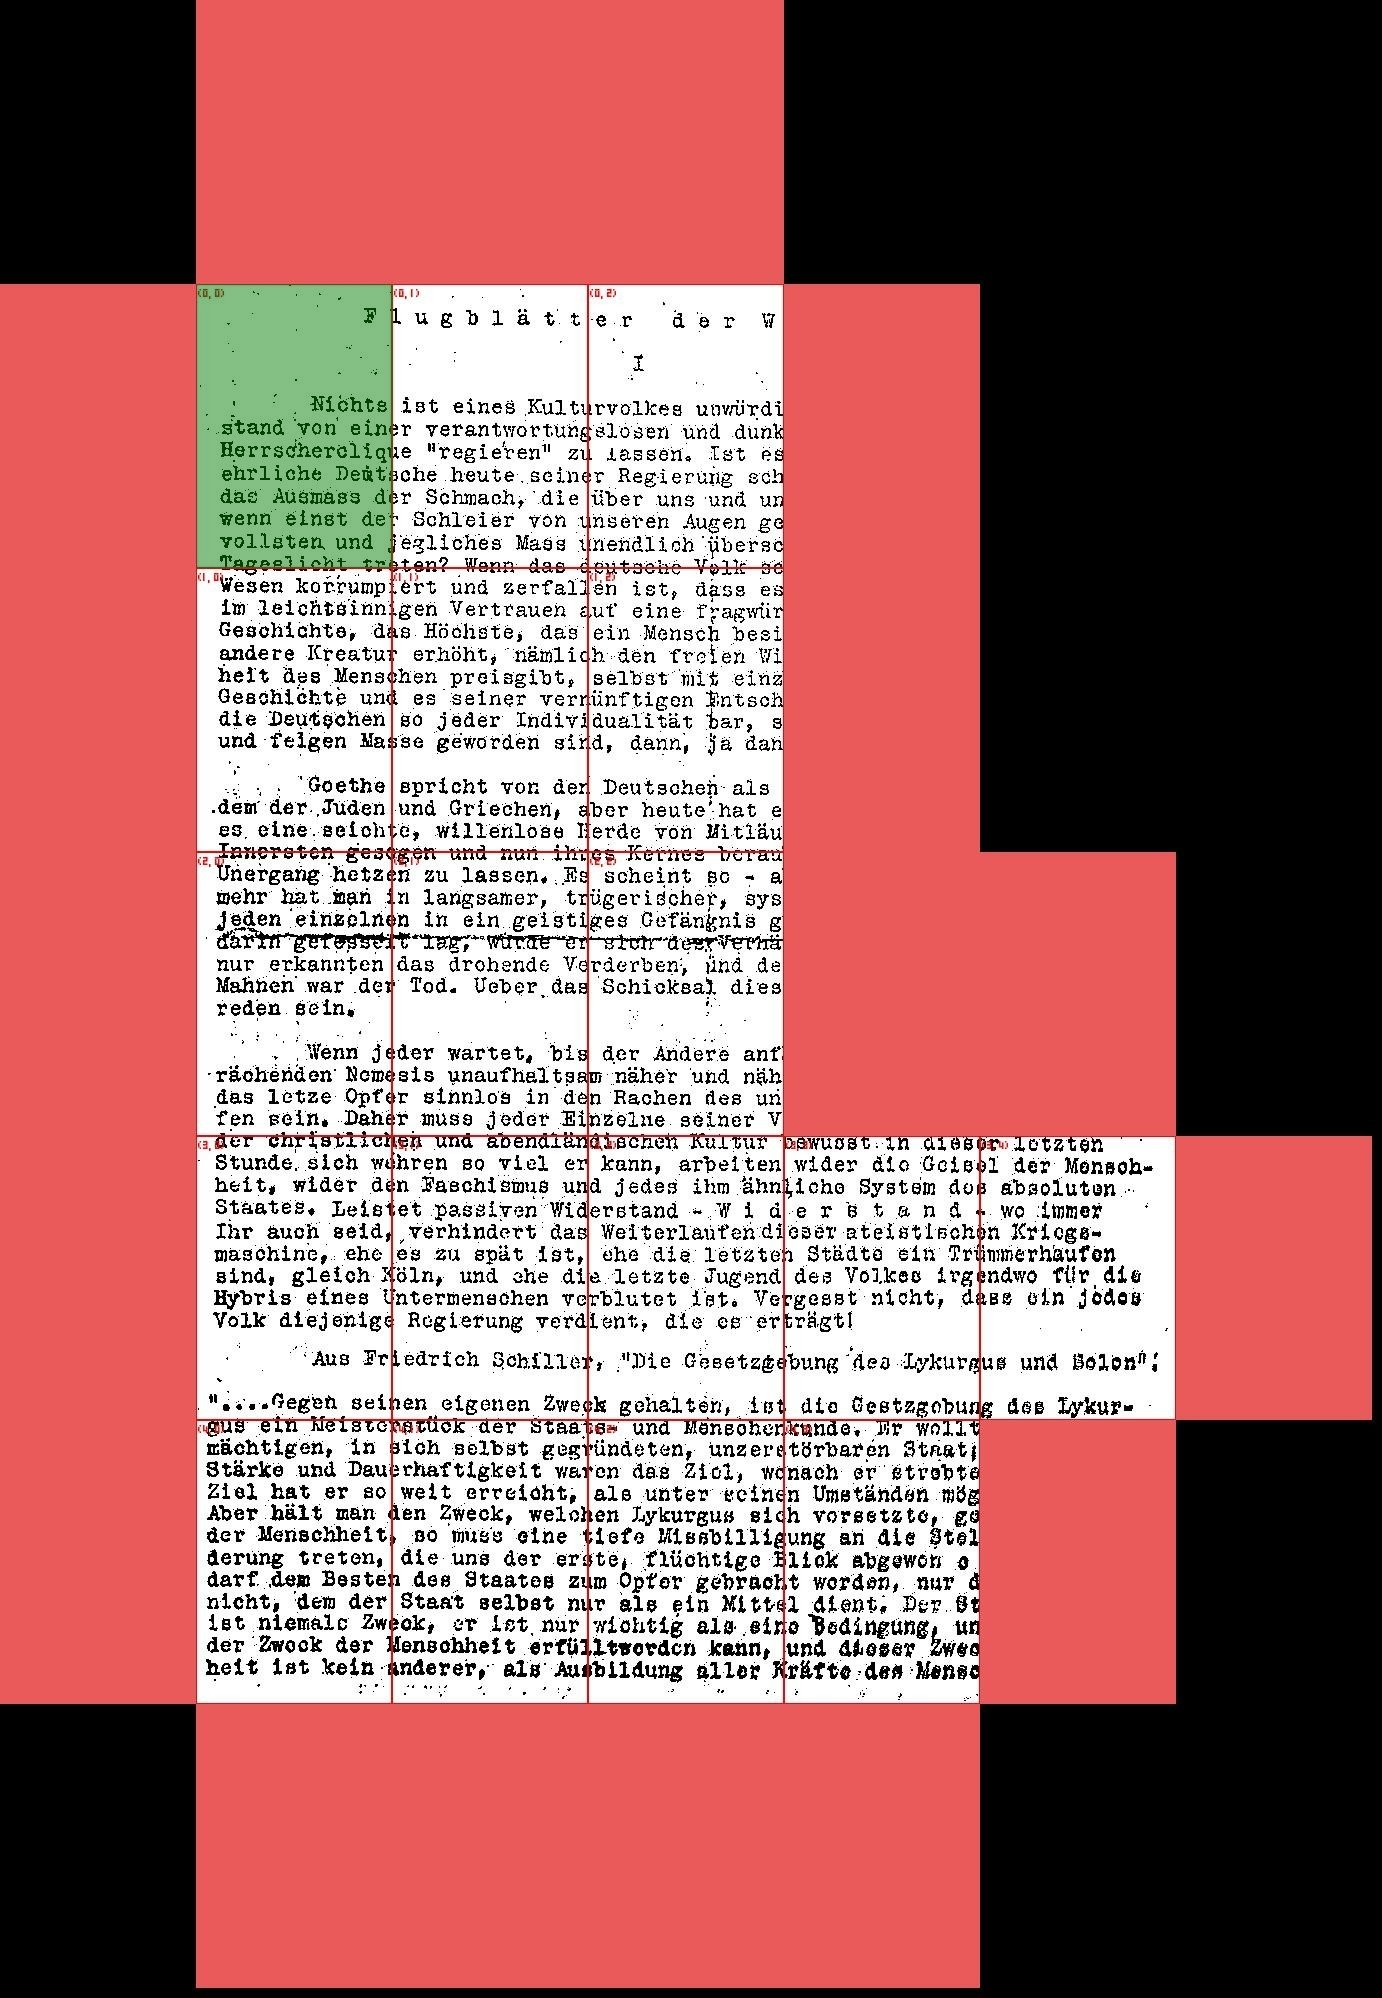
\includegraphics[width=\textwidth]{prim2}
                \vspace{0.3em}
        \end{subfigure}
        ~ 
        \begin{subfigure}[b]{0.45\textwidth}
                \centering
                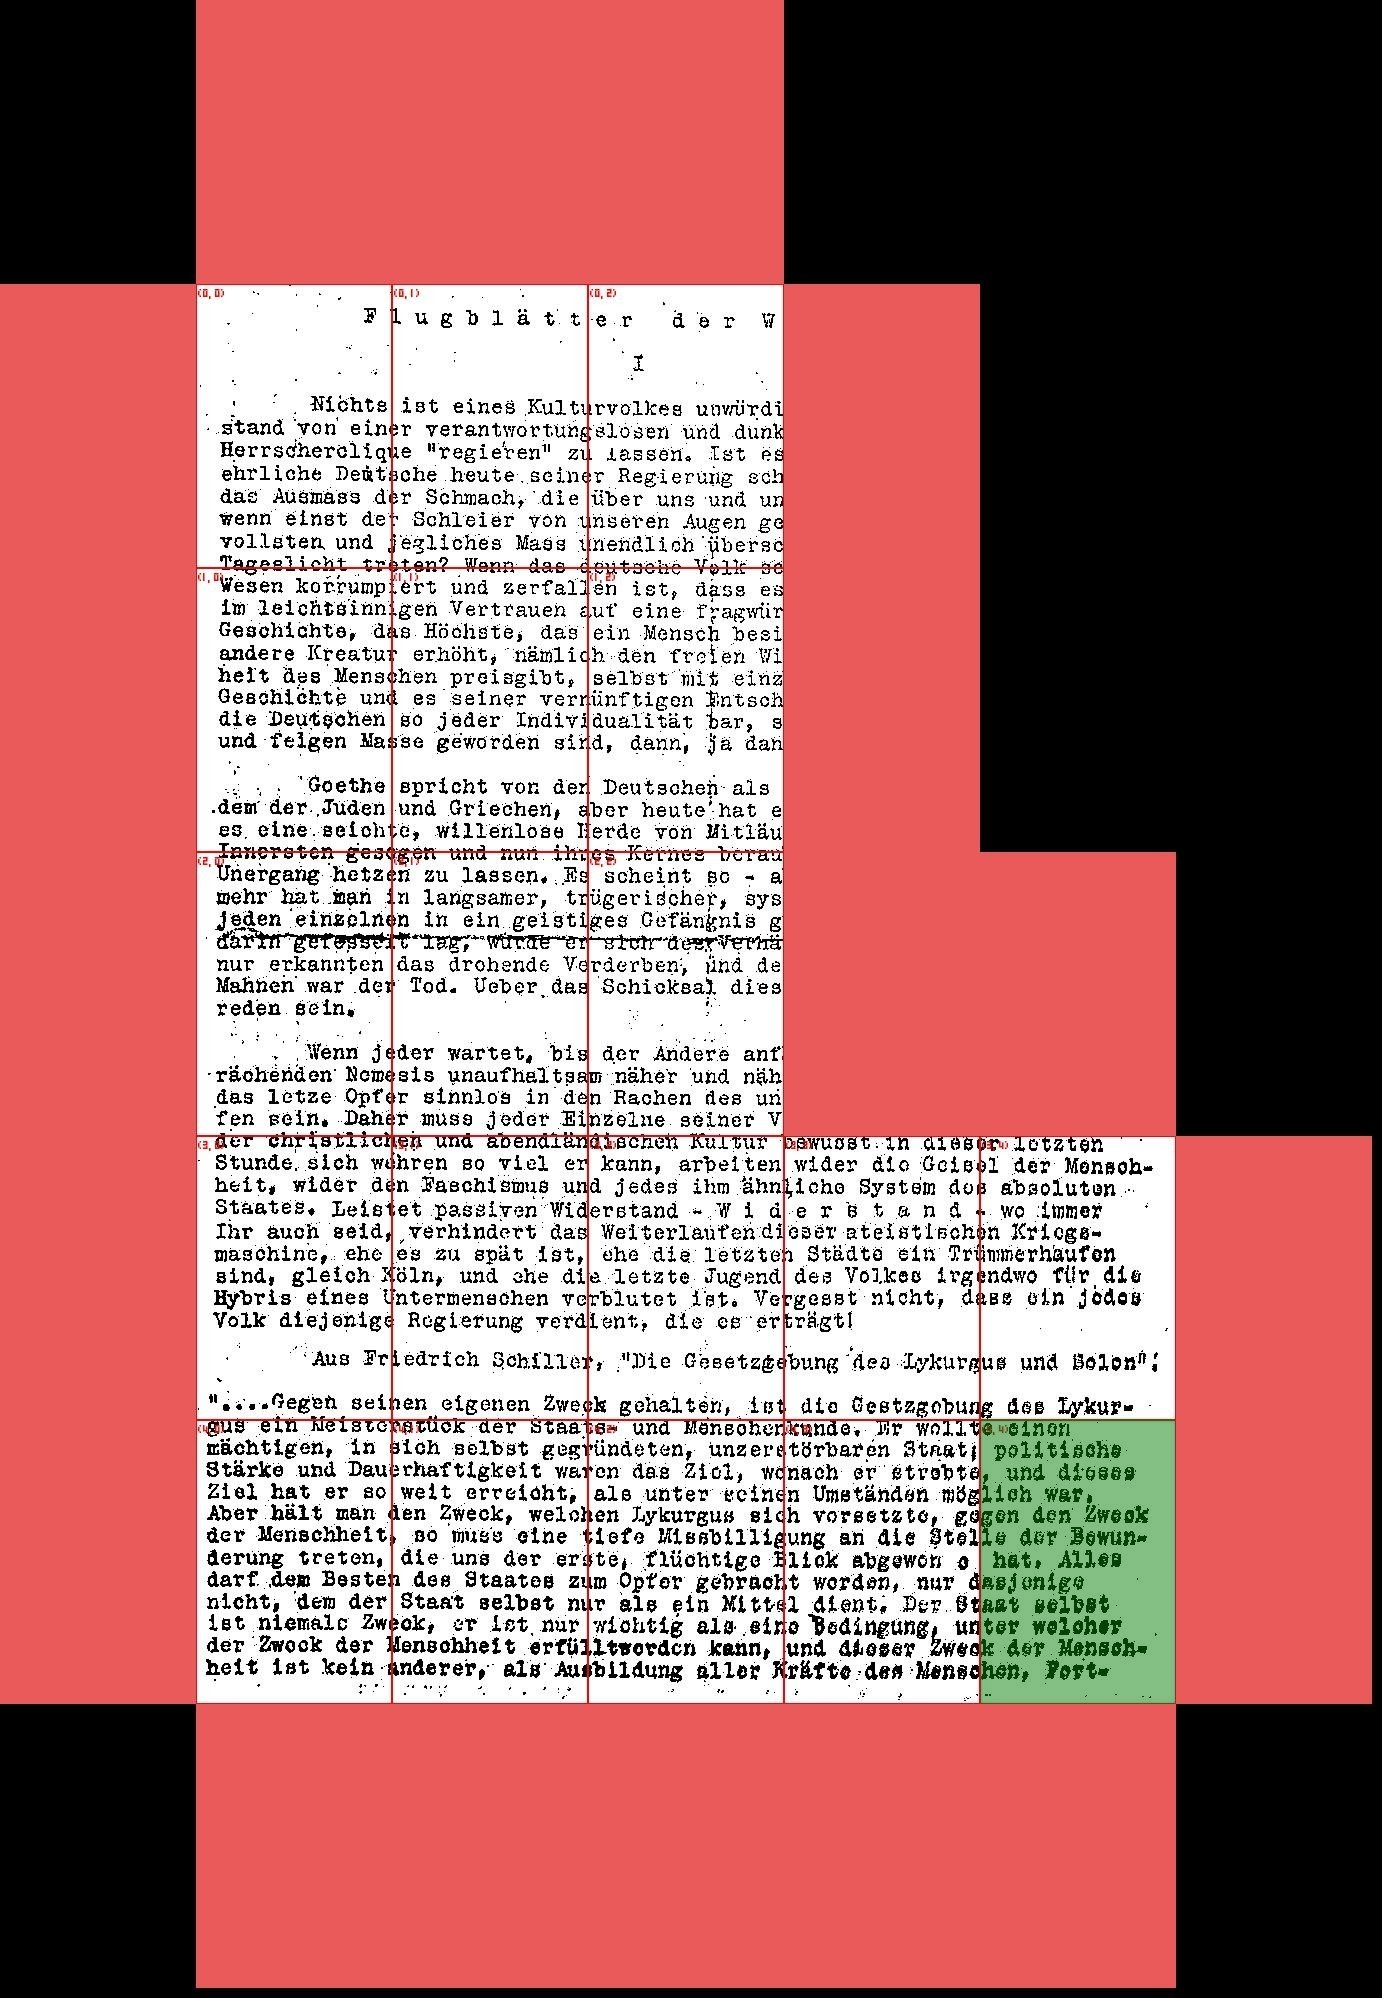
\includegraphics[width=\textwidth]{prim3}
        \end{subfigure}
        ~ 
        \begin{subfigure}[b]{0.45\textwidth}
                \centering
                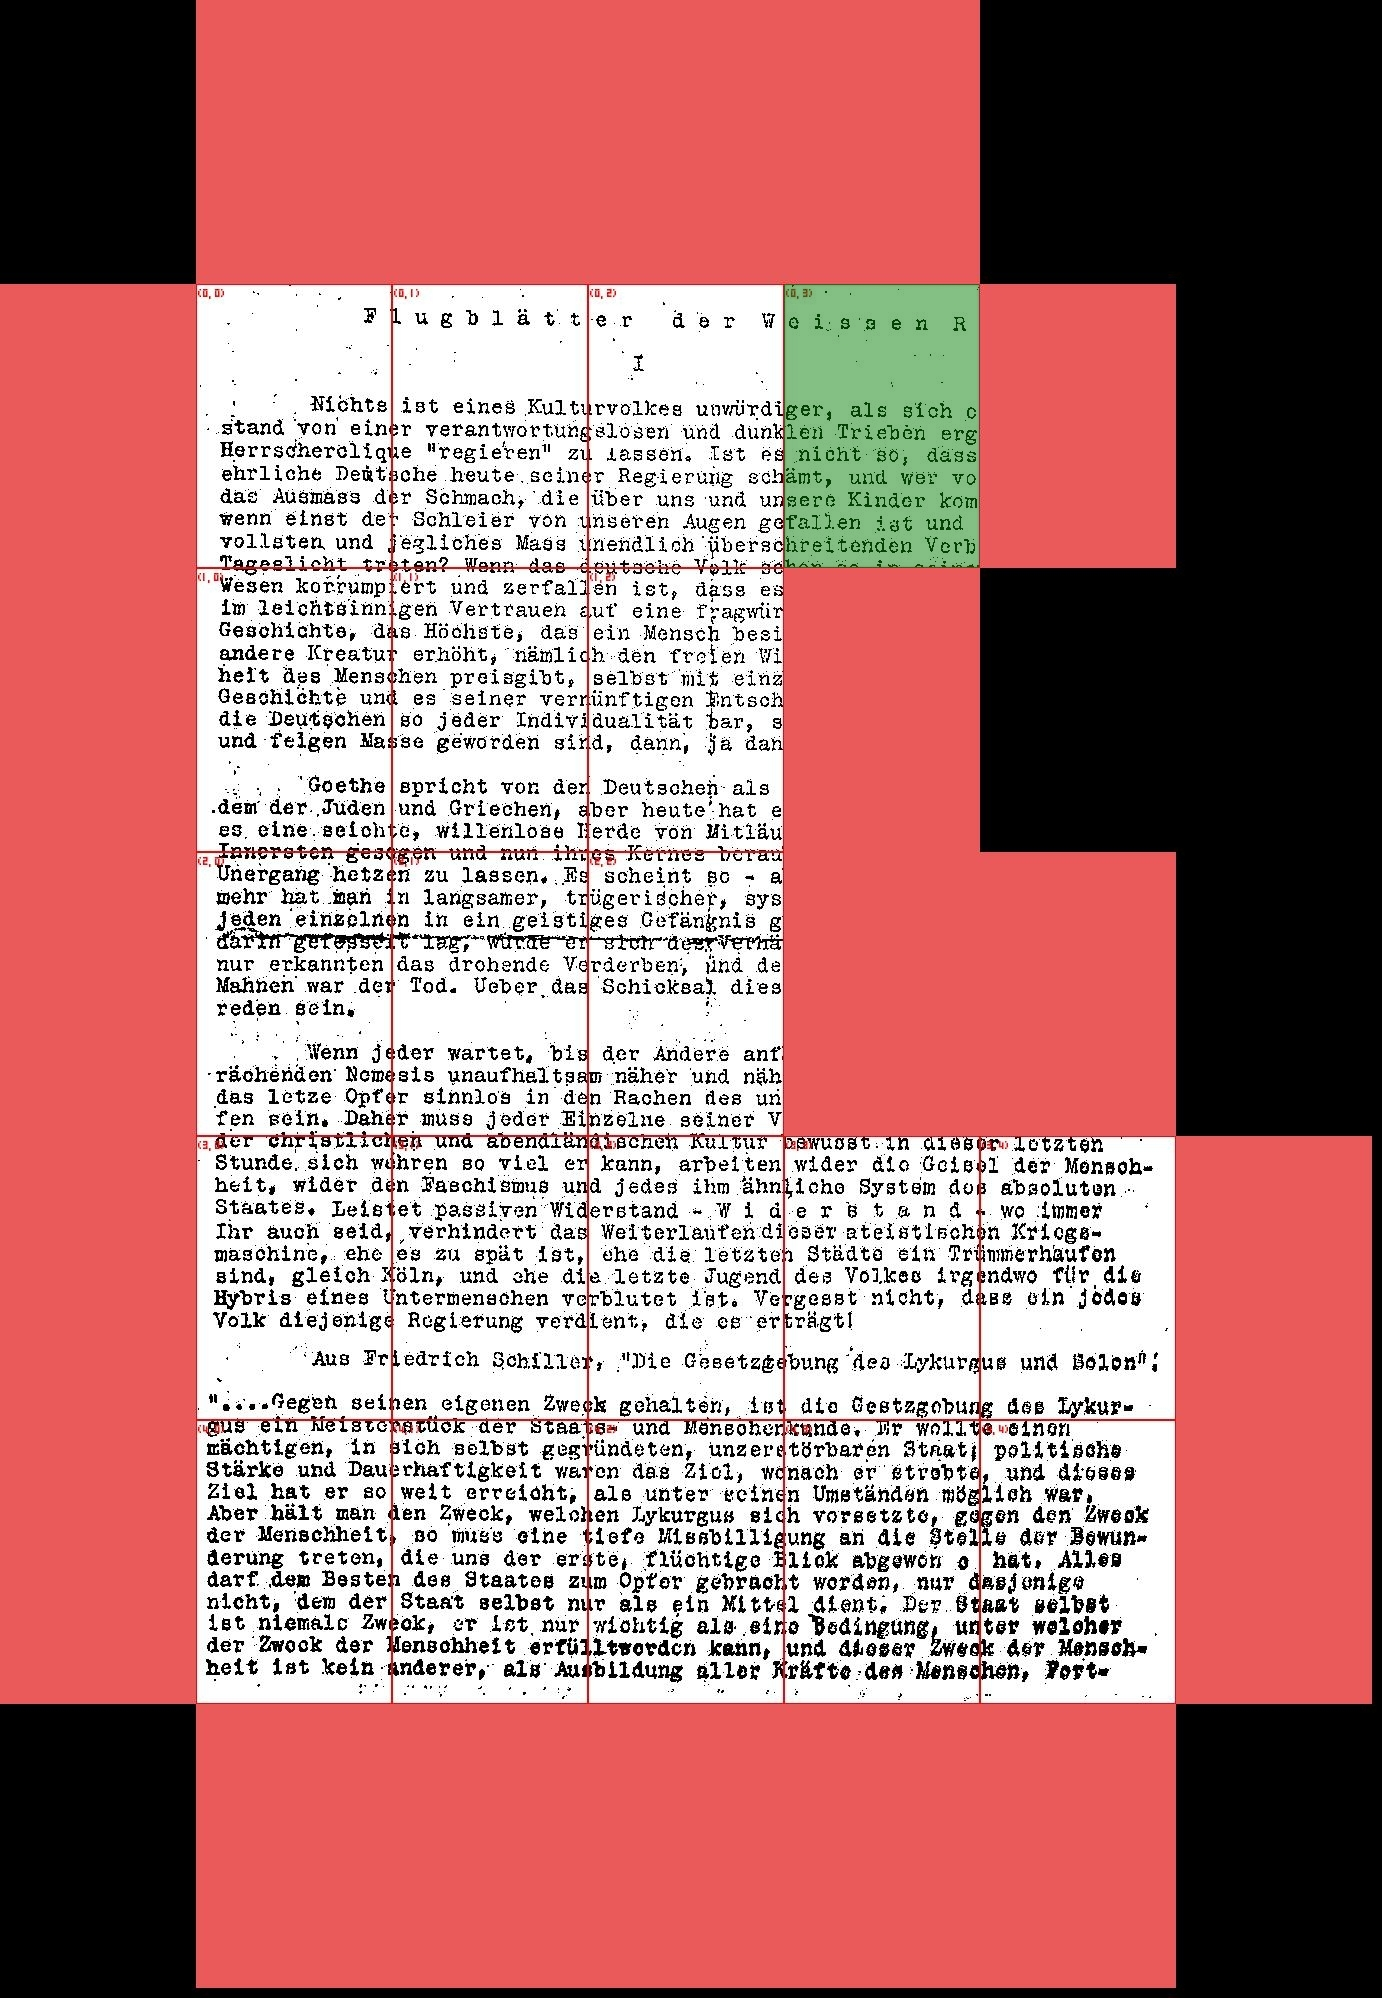
\includegraphics[width=\textwidth]{prim4}
        \end{subfigure}
        \caption{Four steps from the middle of a Prim search are shown. The green pieces highlight the changes that occur in every step and the red pieces show the positions that are considered for the insertion of new shreds.}
        \label{fig:prim}
\end{figure}
Lastly, a heuristic called \emph{ReconstructShreds} is proposed in \cite{P2}. This heuristic can be viewed as a relaxation of the Prim heuristic such that we can have multiple clusters of pieces at any time. ReconstructShreds is looked at in more detail in Section \ref{chap5Desc}.

\section{Pre-processing the shreds}
\label{chap3PP}
As discussed in Section \ref{chap2Ass}, a pre-processing step is needed in order to transform the real, noisy, input into a form suitable for the rest of the algorithm. Several aspects of this pre-processing step have been previously analysed in literature, namely: segmentation, skew correction, up/down orientation and clustering.

\textbf{Segmentation:} The first issue is to actually extract the shreds from the scanned image and to make sure they're all the same size. Skeoch \cite{P26} tackles this problem by first thresholding the original image as to detect the position of the pixels sufficiently different from the background colour. Several ways of automating the threshold selection method are analysed but ultimately, due to the high variance present in scanned images, user input is still required. After thresholding, Skeoch fits rectangles to all pixel blobs over a certain size and thus obtains the individual shreds. A complication can arise when processing narrow strip-cut documents as the shreds can have a tendency to curve, in a manner similar to human hair. Since this curvature can trip up the rectangle fitting, Skeoch proposes instead to detect the corners of the shreds and then fit a polynomial to the edges. An alternative that may be preferable if noise is a major issue, would be to use the Generalised Hough Transform \cite{P44} to detect the delimitation of each shred.

\textbf{Skew Correction:} If we have already detected the shred's bounding rectangles, then fixing the skew of the image can be done by rotating the rectangles so that their longest side is vertical. Alternatively, in \cite{P34} the authors take a different approach by fixing the skew first. They frame the skew correction as an optimization problem and seek the rotation that would minimize the distance between each shred pixel and a vertical line. This completely avoids the need to fit or detect the lines of the shreds since, after the shred has been oriented vertically, a simple bounding box can be taken around it. Both approaches work reasonably well in practice, with maximum errors in the range of 1-2 degrees.

If accuracies greater than this are required, then more complex document orientation methods can be employed. For instance, in \cite{P41}, the authors use a row detection method and then predict the skew and orientation based on some features of these rows. Their method has a precision of 0.1 degrees, and similar results have also been obtained by several other algorithms (eg: \cite{P42,P43}). However none of these methods have been tested on extremely small shreds. Their performance degradation as the information on a shred decreases is unclear and may pose a problem.

\textbf{Up/Down Orientation:} If we have opted for the simpler methods of performing skew correction, then the shreds will now be either correctly oriented or rotated by 180 degrees. Several reliable methods have been developed to deal with this problem. If we restrict the problem to documents written in Roman script, then a robust method is presented in \cite{P45}. The author obtains 100\% accuracy even on documents degraded by noise. Additionally, the method is employed for shred orientation detection in \cite{P32}, thus showing the method can handle orientation on smaller pieces of text (though that paper handles hand-torn documents, so the shreds they look at aren't as small as the ones we might be interested in). For a completely general approach, there are also several orientation methods that work on both Roman and non-Roman scripts, usually by employing some learning algorithm (eg: \cite{P46})

\textbf{Clustering:} One last pre-processing task, useful in some domains, involves clustering the shreds. The problem is that often the shreds of many different documents will be mixed together, thus making the reconstruction process intractable. However, if not all the documents are completely uniform, then the search space can be reduced by clustering the shreds into similar document classes. Several image features have been proposed for this classification task. In \cite{P47}, the authors propose the use of the MPEG-7 standard descriptors \cite{P48} and look at the effectiveness of features such as colour, shape and texture. The paper shows encouraging results for coloured pages, but black and white documents prove to be a harder problem. Their method is expanded upon in \cite{P49}, where in addition to the MPEG-7 descriptors, the authors also detect higher level features, such as whether the paper is from a notebook, by using the Hough transform \cite{P50}. In \cite{P32} the authors propose several other custom features, such as detecting whether the text is typed or handwritten and detecting the type of paper used. For text documents, good results are obtained if the text or paper colour varies, or if the writing changes from typed to handwritten. Making use of subtler features, such as differences in fonts, proved to be more difficult.
